% abtex2-modelo-trabalho-academico.tex, v-1.9.2 laurocesar
%% Copyright 2012-2014 by abnTeX2 group at http://abntex2.googlecode.com/
%%
%% This work may be distributed and/or modified under the
%% conditions of the LaTeX Project Public License, either version 1.3
%% of this license or (at your option) any later version.
%% The latest version of this license is in
%%   http://www.latex-project.org/lppl.txt
%% and version 1.3 or later is part of all distributions of LaTeX
%% version 2005/12/01 or later.
%%
%% This work has the LPPL maintenance status `maintained'.
%%
%% The Current Maintainer of this work is the abnTeX2 team, led
%% by Lauro César Araujo. Further information are available on
%% http://abntex2.googlecode.com/
%%
%% This work consists of the files abntex2-modelo-trabalho-academico.tex,
%% abntex2-modelo-include-comandos and abntex2-modelo-references.bib
%%

% ------------------------------------------------------------------------
% ------------------------------------------------------------------------
% abnTeX2: Modelo de Trabalho Academico (tese de doutorado, dissertacao de
% mestrado e trabalhos monograficos em geral) em conformidade com
% ABNT NBR 14724:2011: Informacao e documentacao - Trabalhos academicos -
% Apresentacao
% ------------------------------------------------------------------------
% ------------------------------------------------------------------------

\documentclass[
	% -- opções da classe memoir --
	12pt,				% tamanho da fonte
	openright,			% capítulos começam em pág ímpar (insere página vazia caso preciso)
	twoside,			% para impressão em verso e anverso. Oposto a oneside
	a4paper,			% tamanho do papel.
	% -- opções da classe abntex2 --
	%chapter=TITLE,		% títulos de capítulos convertidos em letras maiúsculas
	%section=TITLE,		% títulos de seções convertidos em letras maiúsculas
	%subsection=TITLE,	% títulos de subseções convertidos em letras maiúsculas
	%subsubsection=TITLE,% títulos de subsubseções convertidos em letras maiúsculas
	% -- opções do pacote babel --
	english,			% idioma adicional para hifenização
	brazil				% o último idioma é o principal do documento
	]{abntex2}

% ---
% Pacotes básicos
% ---
\usepackage{lmodern}			% Usa a fonte Latin Modern
\usepackage[T1]{fontenc}		% Selecao de codigos de fonte.
\usepackage[utf8]{inputenc}		% Codificacao do documento (conversão automática dos acentos)
\usepackage{lastpage}			% Usado pela Ficha catalográfica
\usepackage{indentfirst}		% Indenta o primeiro parágrafo de cada seção.
\usepackage{color}				% Controle das cores
\usepackage{graphicx}			% Inclusão de gráficos
\usepackage{microtype} 			% para melhorias de justificação
% ---

% ---
% Pacotes adicionais, usados apenas no âmbito do Modelo Canônico do abnteX2
% ---
% Pacotes de citações
% ---
\usepackage[brazilian,hyperpageref]{backref}	 % Paginas com as citações na bibl
\usepackage[alf]{abntex2cite}	% Citações padrão ABNT

% ---
% CONFIGURAÇÕES DE PACOTES
% ---

% ---
% Configurações do pacote backref
% Usado sem a opção hyperpageref de backref
\renewcommand{\backrefpagesname}{Citado na(s) página(s):~}
% Texto padrão antes do número das páginas
\renewcommand{\backref}{}
% Define os textos da citação
\renewcommand*{\backrefalt}[4]{
	\ifcase #1 %
		Nenhuma citação no texto.%
	\or
		Citado na página #2.%
	\else
		Citado #1 vezes nas páginas #2.%
	\fi}%
% ---

% ---
% Informações de dados para CAPA e FOLHA DE ROSTO
% ---
\titulo{Software de alta escalabilidade, performance e disponibilidade aplicada a venda de ingressos online}
\autor{André Formento \and Danilo Hércules Araújo Sousa}
\local{Brasil}
\data{2017, v0.0.5}

\orientador{Nome do professor}
\instituicao{%
  Centro Universitário IBTA
  \par
  Engenharia da computação}
\tipotrabalho{Trabalho de conclusão de curso}
% O preambulo deve conter o tipo do trabalho, o objetivo,
% o nome da instituição e a área de concentração
\preambulo{Monografia apresentada ao Curso de Engenharia da Computação do Centro Universitário IBTA como parte dos requisitos para obtenção de Grau em Engenheiro da Computação.}
% ---


% ---
% Configurações de aparência do PDF final

% alterando o aspecto da cor azul
\definecolor{blue}{RGB}{41,5,195}

% informações do PDF
\makeatletter
\hypersetup{
     	%pagebackref=true,
		pdftitle={\@title},
		pdfauthor={\@author},
    	pdfsubject={\imprimirpreambulo},
	    pdfcreator={LaTeX with abnTeX2},
		pdfkeywords={abnt}{latex}{abntex}{abntex2}{trabalho acadêmico},
		colorlinks=true,       		% false: boxed links; true: colored links
    	linkcolor=blue,          	% color of internal links
    	citecolor=blue,        		% color of links to bibliography
    	filecolor=magenta,      		% color of file links
		urlcolor=blue,
		bookmarksdepth=4
}
\makeatother
% ---

% ---
% Espaçamentos entre linhas e parágrafos
% ---

% O tamanho do parágrafo é dado por:
\setlength{\parindent}{1.3cm}

% Controle do espaçamento entre um parágrafo e outro:
\setlength{\parskip}{0.2cm}  % tente também \onelineskip

% ---
% compila o indice
% ---
\makeindex
% ---

% ----
% Início do documento
% ----
\begin{document}

% Retira espaço extra obsoleto entre as frases.
\frenchspacing

% ----------------------------------------------------------
% ELEMENTOS PRÉ-TEXTUAIS
% ----------------------------------------------------------
% \pretextual

% ---
% Capa
% ---
\imprimircapa
% ---

% ---
% Folha de rosto
% (o * indica que haverá a ficha bibliográfica)
% ---
\imprimirfolhaderosto*
% ---

% ---
% Inserir folha de aprovação
% ---

% Isto é um exemplo de Folha de aprovação, elemento obrigatório da NBR
% 14724/2011 (seção 4.2.1.3). Você pode utilizar este modelo até a aprovação
% do trabalho. Após isso, substitua todo o conteúdo deste arquivo por uma
% imagem da página assinada pela banca com o comando abaixo:
%
% \includepdf{folhadeaprovacao_final.pdf}
%
\begin{folhadeaprovacao}

	\begin{center}
	{\ABNTEXchapterfont\large\imprimirautor}

	\vspace*{\fill}\vspace*{\fill}
	\begin{center}
		\ABNTEXchapterfont\bfseries\Large\imprimirtitulo
	\end{center}
	\vspace*{\fill}

	\hspace{.45\textwidth}
	\begin{minipage}{.5\textwidth}
		\imprimirpreambulo
	\end{minipage}%
	\vspace*{\fill}
	\end{center}

	Trabalho aprovado. \imprimirlocal, 20 de dezembro de 2017:

	\assinatura{\textbf{\imprimirorientador} \\ Orientador}
	\assinatura{\textbf{Professor} \\ Convidado 1}
	\assinatura{\textbf{Professor} \\ Convidado 2}

	\begin{center}
	\vspace*{0.5cm}
	{\large\imprimirlocal}
	\par
	{\large\imprimirdata}
	\vspace*{1cm}
	\end{center}

\end{folhadeaprovacao}
% ---

% Isto é um exemplo de Ficha Catalográfica, ou ``Dados internacionais de
% catalogação-na-publicação''. Você pode utilizar este modelo como referência.
% Porém, provavelmente a biblioteca da sua universidade lhe fornecerá um PDF
% com a ficha catalográfica definitiva após a defesa do trabalho. Quando estiver
% com o documento, salve-o como PDF no diretório do seu projeto e substitua todo
% o conteúdo de implementação deste arquivo pelo comando abaixo:
%
% \begin{fichacatalografica}
%     \includepdf{fig_ficha_catalografica.pdf}
% \end{fichacatalografica}
\begin{fichacatalografica}
	\vspace*{\fill}					% Posição vertical
	\hrule							% Linha horizontal
	\begin{center}					% Minipage Centralizado
	\begin{minipage}[c]{12.5cm}		% Largura

	\imprimirautor

	\hspace{0.5cm} \imprimirtitulo  / \imprimirautor. --
	\imprimirlocal, \imprimirdata-

	\hspace{0.5cm} \imprimirorientadorRotulo~\imprimirorientador\\

	\hspace{0.5cm}
	\parbox[t]{\textwidth}{\imprimirtipotrabalho~--~\imprimirinstituicao,
	\imprimirdata.}\\

	\hspace{0.5cm}
		1. Software
		2. Escalabilidade
		3. Performance
		4. Sistema web.
		5. Microserviço.
		I. Orientador: \imprimirorientador.
		II. \imprimirinstituicao.
		III. \imprimirtitulo.\\

	\hspace{8.75cm} CDU 02:141:005.7\\

	\end{minipage}
	\end{center}
	\hrule
\end{fichacatalografica}
% ---

% isso aqui faz com que o sumário não quebre
% se remover ele gera -2 (menos 2) no número da página
\vspace{\onelineskip}


% resumo em português
\setlength{\absparsep}{18pt} % ajusta o espaçamento dos parágrafos do resumo
\begin{resumo}

  % https://blog.mettzer.com/resumo-abstract-tcc/

  Quando um sistema de ingressos abre as vendas para o público é comum
  que haja muita demanda, ou seja, um pico de requisições.
  Este trabalho apresenta uma abordagem com microsserviços para tratar
  especificamente do processo de reserva de ingressos.
  O objetivo é tornar a arquitetura elástica para que nesses momentos
  de grande demanda mais recursos fiquem disponíveis;
  e, quando a demanda for reduzida, haja otimização -
  garantindo assim escalabilidade, performance e disponibilidade.
  A conclusão mostra que a abordagem de microsserviços garantiu a
  abstração da camada de software, enquanto que a utilização de
  ferramentas adequadas permitiu a abstração da camada de hardware,
  e também, que toda a infraestrutura seja implantada em nuvem.
  Porém, as métricas mostraram que o serviço degradou-se ao receber muitas requisições.

  \textbf{Palavras-chaves}: Escalabilidade, Performance, Disponibilidade, Microsserviço

% escalabilidade
% performance
% disponibilidade
% microsserviço
% resultado
% balanceamento de cargas
% nuvem

\end{resumo}

% resumo em inglês
\begin{resumo}[Abstract]
 \begin{otherlanguage*}{english}
   When a ticket system opens the sales to the public is common
   that there is a lot of demand, that is, a peak of requisitions.
   This work presents a microservice approach to treat
   specifically the ticket reservation process.
   The goal is to make the architecture elastic so that in those moments
   demand more resources become available;
   and, when demand is reduced, there is optimization -
   ensuring scalability, performance and availability.
   The conclusion shows that the microservice approach has
   abstraction of the software layer, while the use of
   appropriate tools allowed the abstraction of the hardware layer,
   and also that the entire infrastructure be deployed in the cloud.
   However, the metrics showed that the service degraded upon receiving many requests.

   \vspace{\onelineskip}

   \noindent
   \textbf{Key-words}: Scalability, Performance, Availability, Microservice
 \end{otherlanguage*}
\end{resumo}


% lista de ilustrações
\pdfbookmark[0]{\listfigurename}{lof}
\listoffigures*
\cleardoublepage

\begin{siglas}
    \item[S\&P 500] Índice de mercado de ações composto por
                    quinhentas empresas diferentes conforme definido
                    por Kennon \cite{definicao-de-sp500}

    \item[Cliente web] É quem consome algum recurso da aplicação

    \item[JSON] JavaScript Object Notation ou Notação de Objetos JavaScript -
                é um formato legível para seres humandos e leve para ser trafegado \cite{define-json}

    \item[URL] Uniform Resource Locator ou Localizador Padrão de Recursos - é o formato de atribuição
               universal para designar um recurso na Internet \cite{define-url}
               
    \item[HTTP] O protocolo de transferência de hipertexto (HTTP) é um protocolo de camada de aplicação
               para transmissão de documentos hipermídia, como HTML. Ele foi projetado para comunicação
               entre navegadores e servidores web, mas também pode ser usado para outros fins \cite{define-http}
               
    \item[POST] Método HTTP. Na requisição HTTP em que é feita utilizando o método POST é possível enviar um anexo \cite{define-post}.
\end{siglas}


% sumario
\pdfbookmark[0]{\contentsname}{toc}
\tableofcontents*
\cleardoublepage

% ----------------------------------------------------------
% ELEMENTOS TEXTUAIS
% ----------------------------------------------------------
\textual

% regra de nome de arquivo:
% antes do _ está o nome da parte
% depois do _ está o nome do capítulo
% os nomes não devem ter espaços, caracteres especiais e devem ser separados por hífen


\chapter*[Introdução]{Introdução}
\addcontentsline{toc}{chapter}{Introdução}

Escrever introdução

\chapter{Problema}

Atualmente a venda de ingressos para eventos ocorre em websites.
O comum é que haja muita divulgação na mídia a respeito do evento.
A venda de ingressos costuma ser muito disputada devido a limitação
física que o local onde ocorrerá permite, assim como, a oferta de
lugares privilegiados, ingressos com descontos (estudante, idoso), etc.
Desta forma, muitas pessoas buscam os ingressos logo após o início das
vendas, gerando uma demanda muito alta nas primeiras horas de venda.

Conforme \cite{10-motivos-para-vender-online}, os compradores consideram
vários motivos para fazer sua compra online, como comodidade por não
precisar ir até um ponto de venda; não enfretam fila; segurança; etc.

\index{alíneas}\index{subalíneas}\index{incisos}A venda de ingressos online
tem diversas temas a serem tratados. Porém, este documento abordará a parte
técnica do sistema focando nos seguintes itens que atenderá alta demanda:

\begin{alineas}

  \item Performance

  \begin{alineas}
     \item sites que não estão preparados para ter grande variação de tráfego
           tendem a ter problemas de performance ou lentidão
  \end{alineas}

  \item Escalabilidade

  \begin{alineas}
     \item vertical: aumento da capacidade computacional de cada equipamento.
           Há limitações físicas de escalabilidade e por isso não é aplicável
           para a solução final.
           Será abordado no trabalho somente a título de comparação.
     \item horizontal: aumento da quantidade de equipamentos
           (podendo manter o mesmo tipo de equipamento). Custo reduzido e
           disponibilidade escalável
     \item Motivação: possibilidade de distrubuição da execução da aplicação para satisfazer
           vários volumes de transação \cite{arquiteturas-em-n-camadas}
  \end{alineas}

  \item Disponibilidade

  \begin{alineas}
     \item quando não planejada, a alta demanda inesperada pode causar até mesmo
           indisponibilidade do sistema, fazendo com que fique temporariamente
           fora do ar;
     \item indisponibilidade causa perda de vendas. Segundo
           \cite{disponibilidade-downtime-perdas}, uma queda no serviço S3 da
           Amazon gerou um prejuízo estimado de \$160.000,00 somente nas empresas
           da S\&P 500
  \end{alineas}

\end{alineas}

\chapter{Objetivos}

\subsection{Objetivo Geral}

\subsection{Objetivos específicos}


\part{Desenvolvimento}

\chapter{Balanceador de carga}

Balanceamento de carga é uma técnica que tem por objetivo a distribuição de carga de trabalho uniformemente entre dois ou
mais computadores. Essa técnica também pode ser utilizada em enlaces de redes e discos rígidos. O mecanismo visa atingir
escalabilidade do sistema e propiciar alta disponibilidade de acesso e respostas de requisições, ou seja, a medida que a
demanda pelos serviços, recursos ou o número de usuários conectados aumentam, mais máquinas são acionadas para incorporar
o conjunto e auxiliar no processamento dos dados.


O balanceamento de rede, consiste na técnica de distribuição de tráfego de rede entre servidores. Essa solução visa entregar
caminhos alternativos a fim de descongestionar os acessos atendendo um número maior de requisições. A segunda geração dos
balanceadores de carga são seguidos pelos sistemas proprietários baseados em aplicativos. Se comportam de forma transparente
as aplicações, ou seja, quando um único servidor não comporta toda carga gerada, é possível iniciar uma nova instância em
outro servidor e balancear a aplicação entre eles.


Utilizando-se do balanceamento de carga, o trabalho propõem tratar um problema que está relacionado com a exponencial
quantidade de requisições recebidas pelos servidores que hospedam sites de vendas de ingresso. A sobrecarga de um
sistema pode ocorrer de maneira linear - com o passar dos anos, por exemplo; ou ainda, exponencial - algum pico de uso
que pode ocorrer com o rápido aumento de requisições em questão de minutos.
No caso do problema da reserva de ingressos, esses picos podem ocorrer regularmente a cada abertura da venda de ingressos.
Com estes pico, cada vez que houver aumento de processamento das requisições e os servidores passarem a entrarem em
estado de sobrecarga, mais servidores podem ser disponibilizados para atenderem a alta demanda e o balanceador de carga
ficaria responsável por distribuir a carga para esses novos servidores também, tornando assim a estrutura escalável
horizontalmente.

O problema poderia demandar uma série de outros problemas para o provedor, isso porque este perderia uma quantidade muita
alta de clientes, muitos desistiriam ou iriam adquirir o produto de outra forma. A confiabilidade da empresa web seria
abalada negativamente, pois diante da frustração, os usuários poderiam passar uma imagem inadequada e que implicaria a perda
de possíveis novos clientes. Consumidores de produtos que compram pela internet, possuem um comportamento que difere em
alguns casos dos compradores de lojas físicas. Eles estão acostumados com um atendimento simples, rápido e sem burocracia.
Quando desejam adquirir algo, seus possíveis vendedores devem oferecer uma experiência que abrange tudo que ele irá
necessitar para comprar o produto, alguma inatividade no site pode significar a perda de uma venda.


Ao que compete a empresa contratante, o provedor do serviço, também sofreria e sua imagem como empresa confiável seria
duramente criticada. A razão pelo efeito dominó está que a única forma de colocar os produtos acessíveis ao público é de
forma virtual. Inconsistências no acesso dos clientes podem ser comparados as portas fechadas de uma loja física.


Sugere-se como uma solução que atende as exigências citadas a utilização de balanceamento de carga baseado em hardware.
Essa tecnologia tem por base dispositivos de rede. Esses diapositivos são neutros em relação aos aplicativos, dessa forma
consegue-se atuar em qualquer plataforma. Em resumo, os componentes oferecem um “servidor virtual” para todos os serviços
que requerem acesso, quando o servidor aceita a requisição, encaminha a mesma para o “servidor real” disponível para atender
e processar os dados. Suas vantagens frente aos demais, é o controle dos servidores, sua disponibilidade, atividade e
operação, monitorado do estado do hardware, isso garante que o sistema irá responder todas as requisições sem perder
desempenho. Com esse gerenciamento também é possível detectar quando os servidores recebem baixo número de acessos, nesse
estado algumas máquinas são desativadas temporariamente, visando economia de energia e preservação dos equipamentos.



\chapter{Resultados da infraestrutura}
%Foi possível demonstrar uma aplicação que escala sob demanda
%Foi apresentada uma arquitetura que é possível de ser aplicada em produção

\section{Uso da infraestrutura}

A escolha da infraestrutura para a solução final foi o uso da
computação em nuvem (\autoref{infraestrutura-em-nuvem}), visto que, proporciona
escalabilidade que o problema exige - uma das principais vantagens da computação em nuvem.
Além é claro, do baixo custo inicial que a aplicação terá antes de começar a gerar qualquer
tipo de lucro.

Conforme discutido a respeito das topologias das plataformas em
nuvem (\autoref{tipologia-das-plataformas-em-nuvem}), para a solução final foi escolhido o
modelo IaaS (\autoref{iaas}) que fornece a opção de rodar programas como Docker e
Kubernetes, tornando a escolha do serviço de plataforma em nuvem independente da forma
com que o software roda. Ou seja, há um desacoplamento da infraestrutura com o software
(\autoref{ferramentas}).

\section{Análise de desempenho}

Foram feitos vários testes em cima do serviço de reserva de ingressos que foi implementado
(\autoref{implementacao-do-servico}) para saber quais eram seus limites.
É importante deixar claro que a análise ocorrera em um notebook pessoal com poder
de processamento limitado, conforme descrito no
\autoref{anexo-especificacao-de-hardware-do-servidor}.
Em um ambiente real (nuvem \autoref{infraestrutura-em-nuvem})
poderão existir diversas máquinas disponíveis para que sejam utilizadas
(escalabilidade horizontal \autoref{escalabilidade})
permitindo que os números exibidos abaixo sejam muito maiores.

\subsection{Gatling: ferramenta para geração da análise de desempenho}

Os testes de perfomance realizados em cima da aplição de reserva de ingressos foram
feitos com a ferramenta Gatling na versão 2.3.
Com a ferramenta é possível testar alta performance de aplicações web
\cite{gatling-docs} que seguem o protocolo HTTP.

\subsection{Gráficos da análises de desempenhos}

O teste de performance de requisições foi feito usando a
estratégia do método heavisideUsers \cite{gatling-simulation-setup}
que o Gatling possui, simulando assim a utilização simultânea do sistema por
grande quantidade de usuários.
As requisições da análise da
\autoref{03000-requests-config-10s-duration-10},
\autoref{05000-requests-config-10s-duration-10}
e \autoref{10000-requests-config-10s-duration-13}
foram configuradas para serem executadas no período de 10 segundos.
Os testes foram feitos para medir a degradação do sistema em relação ao aumento do
número de requisições simulando um ambiente onde haveriam muitas requisições para
reserva de ingressos.
Com a degração do sistema as respostas começam a demorar mais, ou seja,
o teste demora mais para ser finalizado conforme o aumento do número de requisições.
Com isso, o único parâmetro que muda de um teste para o outro
é o número de requisições realizadas.

Na \autoref{03000-requests-config-10s-duration-10} são feitas 3.000 requisições apenas.
O sistema responde todas elas com sucesso e um desvio padrão de 241 milisegundos
para o tempo de resposta das requisições.
97\% das requisições respondem em menos de 800 milisegundos e apenas 3\% das requisições
respondem em até 1.200 milisegundos.

\begin{figure}[h]
  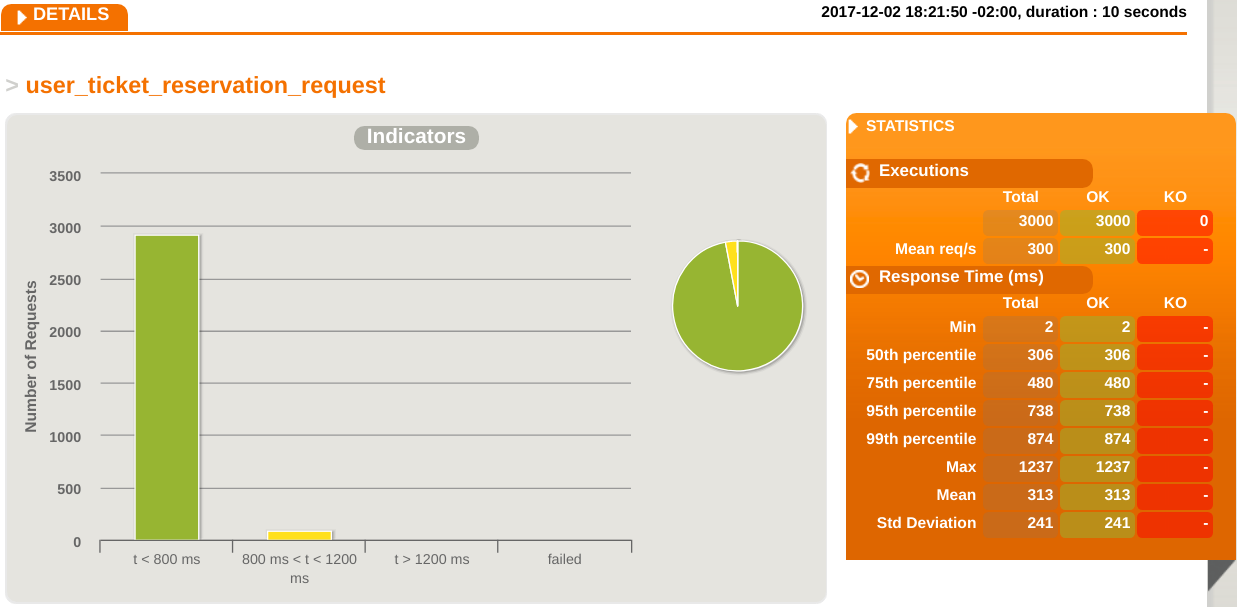
\includegraphics[width=\textwidth]{03000-requests-config-10s-duration-10}
  \caption{Dados do Gatling com 3.000 requisições executados em 10 segundos}
  \label{03000-requests-config-10s-duration-10}
\end{figure}

Na \autoref{05000-requests-config-10s-duration-10} são feitas 5.000 requisições.
O sistema responde todas elas com sucesso e um desvio padrão aumenta para 569 milisegundos
para o tempo de resposta das requisições.
78\% das requisições respondem em menos de 800 milisegundos, 18\% das requisições
respondem em até 1.200 milisegundos e apenas 4\% das requisições
respondem com tempo maior que 1.200 milisegundos.

\begin{figure}[h]
  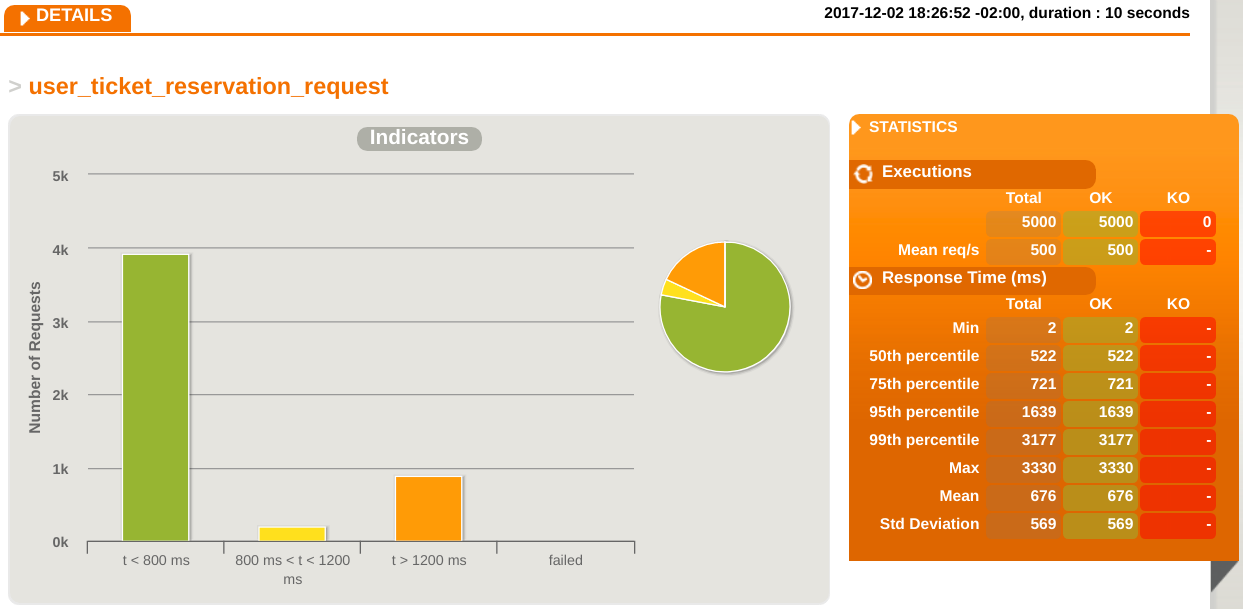
\includegraphics[width=\textwidth]{05000-requests-config-10s-duration-10}
  \caption{Dados do Gatling com 5.000 requisições executados em 10 segundos}
  \label{05000-requests-config-10s-duration-10}
\end{figure}

Na \autoref{10000-requests-config-10s-duration-13} são feitas 10.000 requisições.
O sistema responde todas elas com sucesso e um desvio padrão aumenta para 1117 milisegundos
para o tempo de resposta das requisições.
5\% das requisições respondem em menos de 800 milisegundos, 3\% das requisições
respondem em até 1.200 milisegundos e apenas 93\% das requisições
respondem com tempo maior que 1.200 milisegundos. Aqui fica claro que há grande
degradação do sistema quanto ao tempo de resposta. Porém, o mais importante
é que todas as requisições foram atendidas e o tempo ainda é aceitável para
um ambiente de produção.

\begin{figure}[h]
  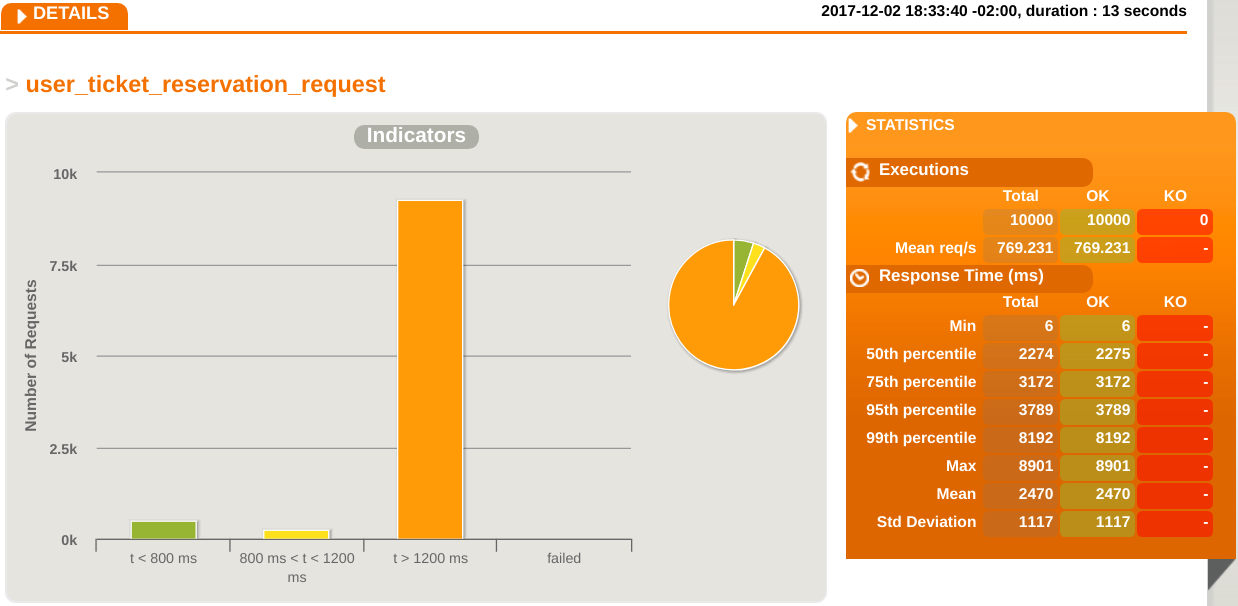
\includegraphics[width=\textwidth]{10000-requests-config-10s-duration-13}
  \caption{Dados do Gatling com 10.000 requisições executados em 13 segundos}
  \label{10000-requests-config-10s-duration-13}
\end{figure}

A \autoref{28000-requests-config-30s-duration-34} possui o tempo de teste configurado
com 30 segundos de execução.
O que se pode concluir com os dados analisados é que a aplicação consegue atender
em torno de 28.000 requests com sucesso em 30 segundos com desvio padrão de
4111 milisegundos.
O tempo de respostas é considerado alto - imaginando um usuário aguardando em
torno de 5 segundos para saber se sua reserva foi realizada.
Porém, a solicitação da reserva é atendida.

Com a escalabilidade horizontal é possível começar a expandir esse poder de processamento.
Com mais máquinas disponíveis o tempo de resposta das aplicações poderia ser reduzido.

\begin{figure}[h]
  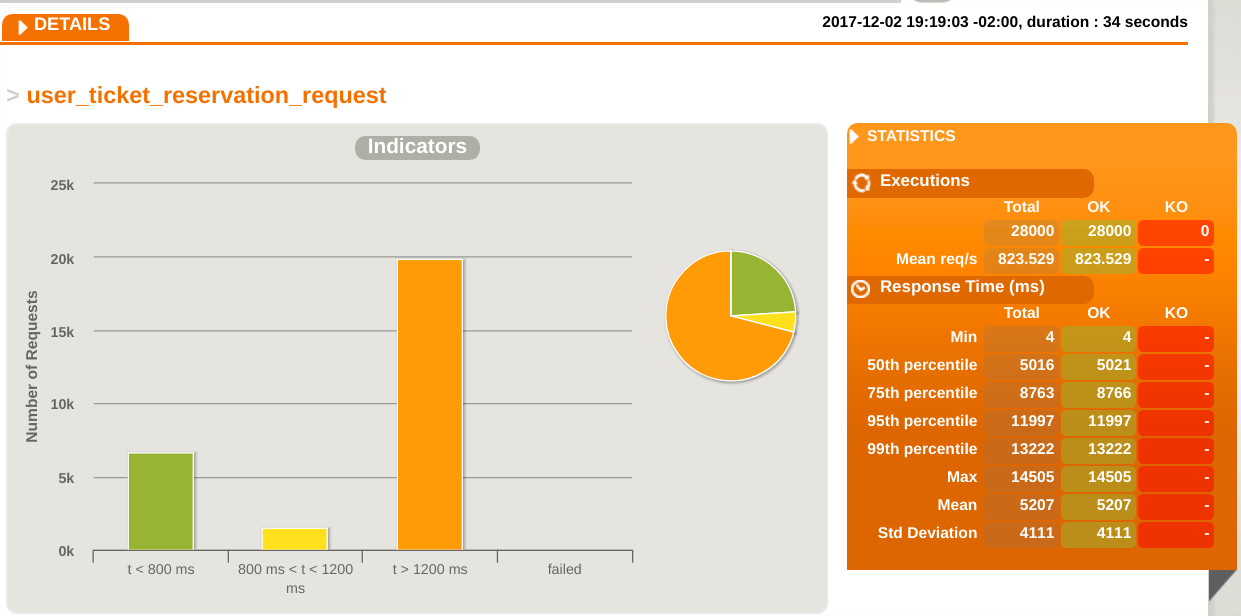
\includegraphics[width=\textwidth]{28000-requests-config-30s-duration-34}
  \caption{Dados do Gatling com 28.000 requisições executados em 34 segundos}
  \label{28000-requests-config-30s-duration-34}
\end{figure}

Todos os resultados com todos os testes realizados pode ser consultados de maneira
iterativa através do link \url{https://andreformento.github.io/term-paper/index.html}.


\chapter*[Conclusão]{Conclusão}
\addcontentsline{toc}{chapter}{Conclusão}

% microserviços
As vantagens que os microseviços trazem foram o motivo da escolha por esta abordagem.
Isso possibilitou separar e implementar apenas uma parte
de uma solução mais geral, que é a venda de ingressos.
Foi possível também que os testes de performance fossem realizados num ponto específico
e deixado claro o comportamento no momento da vendas de ingressos.
Esses dados geram estimativas inclusive para tomadas de decisão quanto aos custos
que uma venda de ingressos pode gerar - e a escolha de qual plataforma utilizar.

% resultados
O resultados apresentados mostram que houve degradação dos serviços com o aumento do
número de requisições.
% escalabilidade / balanceamento de cargas
Porém, usando a abordagem de escalabilidade horizontal e o balanceamento de cargas,
é possível que mais servidores sejam disponibilizados para atender essa alta demanda.

Como o serviço de reserva de ingressos está desacoplado em um serviço de contexto bem
definido, é possível lidar com ele de maneira independente.
% nuvem
Isso em um ambiente de nuvem (IaaS) torna possível a auto escalabilidade com baixo esforço.
Com o uso de ferramentas que auxiliam na implantação, como Docker e Kubernetes,
é possível automatizar o ambiente para que se comporte de maneira otimizada -
quando há grande demanda, vários servidores são disponibilizados, mas no momento
de baixa utilização, várias máquinas podem ser desligadas.
% performance / disponibilidade
Isso influência no desempenho do sistema.
A performance e a disponibilidade é garantida e a degradação é minimizada.

% conclusão final :D
Para o usuário final a experiência de comprar um ingresso em um sistema desses
é positiva, visto que, mesmo que vários outros usuários estão tentando
fazer aquela mesma compra, ele não é afetado e consegue concluir de maneira
satisfatória o processo.


% ----------------------------------------------------------
% Referências bibliográficas
% ----------------------------------------------------------
\bibliography{referencias-bibliograficas}

% ----------------------------------------------------------
% Glossário
% ----------------------------------------------------------
%
% Consulte o manual da classe abntex2 para orientações sobre o glossário.
%
%\glossary

\begin{apendicesenv}
    
    % Imprime uma página indicando o início dos apêndices
    \partapendices
    
    \chapter{Algum apêndice}
    
    escreve sobre algum apêndice
    
    \chapter{Outro apêndice}

    escreve sobre outro apêndice
    
\end{apendicesenv}


\begin{anexosenv}

    % Imprime uma página indicando o início dos anexos
    \partanexos

    \chapter{Especificação de hardware do servidor}

        \index{alíneas}\index{subalíneas}\index{incisos}As especificações de Hardware
        do computador que foram feitos os testes estão descritas nos próximos tópicos.
        Os testes foram realizados em um notebook de uso pessoal.

        \begin{alineas}

        \item CPU

        \begin{alineas}

            \item Arquitetura: x86\_64

            \item Empresa: Intel Corp.

            \item Produto: Intel(R) Core(TM) i7-4.800MQ CPU @ 2,70GHz

            \item Quantidade de núcleos: 8

            \item Frequência padrão: 2.848MHz

            \item Frequência mínima:  800MHz

            \item Frequência máxima: 3.700MHz

            \item Virtualização: VT-x

            \item L1d cache: 32K

            \item L1i cache: 32K

            \item L2 cache: 256K

            \item L3 cache: 6.144K

        \end{alineas}

        \item Memória

        \begin{alineas}

            \item Capacidade por unidade: 8.192 MB

            \item Quantidade: 2

            \item Capacidade total: 16.384 MB

            \item Modelo: SODIMM

            \item Set: None

            \item Tipo: DDR3

            \item Velocidade: 1.600 MT/s

        \end{alineas}

        \item Armazenamento

        \begin{alineas}

            \item Modelo: Samsung SSD 840

            \item Empresa: Samsung

            \item Device: SSD 840

            \item Detalhe: Samsung SSD 840 PRO Series (DXM05B0Q)

            \item Capacdade: 256 GB

        \end{alineas}

        \item Sistema operacional

        \begin{alineas}

            \item Sistema operacional: Linux

            \item Distro: Fedora

            \item Release: 26

            \item Versão do Kernel: 4.13.12-200.fc26.x86\_64

        \end{alineas}

        \end{alineas}

    %\chapter{Outro anexo}

    %escreve outro anexo

\end{anexosenv}


%---------------------------------------------------------------------
% INDICE REMISSIVO
%---------------------------------------------------------------------
%\phantompart
%\printindex
%---------------------------------------------------------------------

\end{document}
